\documentclass[12pt]{article}

% Pacotes básicos
\usepackage[utf8]{inputenc}
\usepackage[T1]{fontenc}
\usepackage[english]{babel}
\usepackage{times}
\usepackage{amsmath}
\usepackage{amsfonts}
\usepackage{amssymb}
\usepackage{graphicx}
\usepackage[margin=2.5cm]{geometry}
\usepackage{setspace}
\usepackage{indentfirst}
\usepackage{caption}
\usepackage{subcaption}
\usepackage{booktabs}
\usepackage{multirow}
\usepackage{float}
\usepackage{cite}
\usepackage{pgfplots}
\usepackage{tikz}
\pgfplotsset{compat=1.18}

%\usepackage[style=apa]{biblatex}
%\addbibresource{referencias.bib}

% Definição de comandos personalizados
\newcommand{\namostras}{Nº de amostras}
\newcommand{\oautor}{o autor}

% Configurações de espaçamento
\onehalfspacing
\setlength{\parindent}{1.25cm}

% Título e autores
\title{\textbf{Multivariate Calibration Modeling: Multiple Linear Regression with Ensemble Methods and Root Mean Square Error of Prediction Evaluation}}

\author{
Wagner Oliveira de Araujo\textsuperscript{a} and Cid Nelson Silva\textsuperscript{a,*}\\
\textsuperscript{a}\textit{Instituto Federal de Educação, Ciência e Tecnologia de Goiás, Campus Anápolis,}\\
\textit{Bacharelado em Ciência da Computação, 75131-457 Anápolis-GO, Brazil}
}

\date{}

\begin{document}

\maketitle

\begin{abstract}
This study evaluates the application of statistical resampling techniques in multivariate calibration applied to chemometrics. Fundamental concepts such as multivariate linear regression (MLR), random sampling, empirical distribution, and the plug-in principle are presented. Two widely used resampling approaches were investigated: bagging and subagging. As a practical application, the simultaneous determination of Mn, Mo, Cr, Ni, and Fe in alloy steel samples was performed using optical emission spectrometry with plasma and photodiode array detection. Model evaluation was based on prediction errors in independent test samples. Results indicated variable performance among methods, depending on the evaluated analyte. The MLR-bagging and MLR-subagging approaches showed significant gains in prediction accuracy for Cr and Fe, demonstrating the effectiveness of ensemble techniques in these contexts. In contrast, classical MLR demonstrated superior performance for Mn, Mo, and Ni, indicating that the additional complexity of ensemble strategies does not result in significant precision improvements for these analytes. Regarding computational cost, MLR-subagging proved to be approximately 2.5 times faster than MLR-bagging, configuring itself as a balanced alternative between precision and efficiency, evidencing its potential in chemometric applications subject to temporal restrictions.
\end{abstract}

\textbf{Keywords:} resampling techniques, multivariate calibration, bagging, subagging, MLR

\section{Introduction}

Multivariate calibration plays a fundamental role in various areas of chemical and industrial analysis, enabling the extraction of valuable information from complex data. In the specific context of alloy steel analysis, precise determination of elemental composition (Mn, Cr, Mo, Ni, Fe) is crucial to ensure the quality and desired properties of the material. However, the complexity of multivariate data from instrumental analysis methods requires the use of advanced statistical techniques to obtain reliable results.\cite{Ewing:1972,Harley:1954,Skoog:1997}

This study investigates the application of resampling techniques (bootstrap), bagging, and subagging in Multiple Linear Regression (MLR) to optimize multivariate calibration of alloy steel samples. The research seeks to fill the knowledge gap regarding the application of these ensemble techniques in this specific context, contributing to the advancement of chemometrics and to the improvement of alloy steel analyses in various sectors.\cite{Pimentel:1998}

The main objective is to analyze and compare the performance of bagging and subagging techniques applied to Multiple Linear Regression (MLR) in multivariate calibration of data from alloy steel samples, aiming to optimize modeling precision and analysis efficiency.

\section{Theoretical Background}

\subsection{Multiple Linear Regression}

MLR is employed when it is necessary to establish a relationship involving more than one independent variable ($x$):

\begin{equation}
y = x_1b_1 + x_2b_2 + \ldots + x_nb_n
\end{equation}

\noindent where $b_j \in \mathbb{R}$, $j = 1, 2, \ldots, n$. In matrix form:

\begin{equation}
y = \mathbf{xb}
\end{equation}

The estimation procedure is called multiple linear regression.\cite{Kramer:1998,Martens:1989} Having calibration data:

\begin{equation}
\{(\mathbf{x}_i, y_i), i = 1, 2, \ldots, M\}
\end{equation}

or in matrix form:

\begin{equation}
\mathbf{X}_{cal} = \begin{bmatrix} \mathbf{x}_1 \\ \mathbf{x}_2 \\ \vdots \\ \mathbf{x}_M \end{bmatrix}, \quad
\mathbf{y}_{cal} = \begin{bmatrix} y_1 \\ y_2 \\ \vdots \\ y_M \end{bmatrix}
\end{equation}

The best estimate in the least squares sense for the coefficient vector $\mathbf{b}$ is given by the Moore-Penrose pseudo-inverse:\cite{Lawson:1974}

\begin{equation}
\hat{\mathbf{b}} = \mathbf{X}^+_{cal}\mathbf{y}_{cal} = (\mathbf{X}^T_{cal}\mathbf{X}_{cal})^{-1}\mathbf{X}^T_{cal}\mathbf{y}_{cal}
\end{equation}

\subsection{Bootstrap Technique}

Statistical inference establishes properties for population $X$ from the analysis of a random sample from that population.\cite{Draper:1998,Johnson:2001,Chatterjee:2006} The bootstrap method is a computational procedure that provides a measure of the precision level of statistical inference, such as mean, standard deviation, and standard error.\cite{Kupper:1998,Stephan:2005} The basic idea of bootstrap is to statistically infer the properties of interest from the analysis of random samples extracted from the original population without the need to know the data distribution a priori, which constitutes a significant advantage over other techniques.

A random sample $\mathbf{x}_{al} = [x_{al1}, \ldots, x_{aln}]$ is extracted from the probability distribution $D$. The parameter of interest $\theta = t(d)$ is unknown and will be estimated based on the observed sample $\mathbf{x}_{al}$, resulting in the estimator $\hat{\theta} = t(\mathbf{x}_{al})$.

\subsubsection{Bootstrap Estimate}

The bootstrap method initially needs bootstrap samples and then applies bootstrap replications. The bootstrap sample is defined as the random sample of size $n$ extracted from the empirical distribution $\hat{d}$, represented by $\mathbf{x}^* = [x^*_1, x^*_2, \ldots, x^*_n]$.\cite{Efron:1994} Bootstrap samples are obtained by resampling with replacement, and there may be repetitions of elements from the original sample.

Bootstrap replications are represented by:

\begin{equation}
\hat{\theta}^* = s(\mathbf{x}^*)
\end{equation}

\noindent where $s(\gamma)$ is the statistical function to be applied to the bootstrap samples.

\subsection{Empirical Distribution Function}

Suppose a random sample of size $n$, given by $\mathbf{x} = \{x_1, x_2, \ldots, x_n\}$, is obtained from a probability distribution function $d$. The empirical distribution function $\hat{d}$ is defined as the discrete distribution that assigns probability $\frac{1}{n}$ to each observed value $x_i$, for $i = 1, 2, \ldots, n$.

In other words, the empirical distribution $\hat{d}$ is constructed from the sample space of $\mathbf{x}$, assigning the following empirical probability to an event $A$:

\begin{equation}
\hat{Pr}\{A\} = \frac{\#\{x_i \in A\}}{n}
\end{equation}

\noindent where $\#\{x_i \in A\}$ denotes the number of observations $x_i$ that belong to set $A$.

\subsection{Plug-in Principle}

The plug-in principle constitutes a fundamental approach for estimating statistical parameters, allowing the estimation of a parameter of interest $\theta$ through an evaluative function applied to the empirical distribution of the data.

Formally, let $\theta = t(F)$ be a parameter defined as a function of the population distribution $F$. The plug-in estimator is obtained by replacing $F$ with the empirical distribution $\hat{F}_n$:

\begin{equation}
\hat{\theta} = t(\hat{F}_n)
\end{equation}

\noindent where $n$ denotes the sample size. It is important to highlight that the bootstrap method constitutes a direct application of the plug-in principle.\cite{Efron:1997,Fernandez:1999}

\subsection{Classical Resampling Techniques}

\subsubsection{Bagging}

The bagging technique (Bootstrap Aggregating) was proposed by Breiman\cite{Breiman:1996} with the objective of generating multiple calibration sets through bootstrap resampling, subsequently combining the obtained results. This approach aims to reduce the variance of the final predictor through aggregation.

Breiman demonstrated that bagging provides significant performance gains in regression problems, especially when the model is unstable – that is, when small changes in the calibration set result in substantial changes in predictions.\cite{Shabbir:2024,Hong:2020}

The bagging algorithm can be summarized as follows:

\begin{enumerate}
\item Define the number of bootstrap replicas $B$
\item For each replica $b = 1, \ldots, B$:
   \begin{itemize}
   \item Generate bootstrap sample $\mathbf{x}^{*(b)}$ of size $n$ with replacement from $\mathbf{x}$
   \item Calculate the statistic for replica $b$: $\hat{\theta}^{*(b)} = s(\mathbf{x}^{*(b)})$
   \end{itemize}
\item Aggregate replicas via arithmetic mean:
\end{enumerate}

\begin{equation}
\hat{\theta}^*_{bag} = \frac{1}{B}\sum_{b=1}^{B}\hat{\theta}^{*(b)}
\end{equation}

\subsubsection{Subagging}

The subagging technique (subsample aggregating) is based on resampling without replacement, differing from traditional bagging by not allowing repetitions of observations within samples.\cite{Silva:2020,Buhlmann:2003} Each model is constructed similarly to bagging, but using reduced-size subsamples $k < n$.

The subagging algorithm follows a structure similar to bagging, but with the fundamental difference that subsamples of size $k$ are generated without replacement from the original data. The aggregation is also performed through the arithmetic mean:

\begin{equation}
\hat{\theta}^*_{subag} = \frac{1}{B}\sum_{b=1}^{B}\hat{\theta}^{*(b)}
\end{equation}

The absence of replacement implies that each observation appears at most once per subsample, fundamentally differentiating this technique from bagging.\cite{Revelas:2024,Qin:2023,Galvao:2006}

\section{Materials and Methods}

\subsection{Alloy Steel Samples}

Data were obtained through a sequential inductively coupled plasma atomic emission spectrometer converted to a multi-channel detection system based on a linear array of 1024 photodiodes, as described by Pimentel et al.\cite{Pimentel:1998}

The instrumental response matrices and concentration of alloy steel samples are organized into two datasets: calibration (66.67\%) and test (33.33\%), as shown in Table~\ref{tab:dimensions}.

\begin{table}[H]
\centering
\caption{Dimensions of datasets for different elements.}
\label{tab:dimensions}
\begin{tabular}{lcc}
\toprule
Element & Calibration & Test \\
\midrule
Mn & $\mathbf{X}_{cal}^{Mn}(34\times723)$, $\mathbf{Y}_{cal}^{Mn}(34\times1)$ & $\mathbf{X}_{test}^{Mn}(17\times723)$, $\mathbf{y}_{test}^{Mn}(17\times1)$ \\
Mo & $\mathbf{X}_{cal}^{Mo}(21\times723)$, $\mathbf{Y}_{cal}^{Mo}(21\times1)$ & $\mathbf{X}_{test}^{Mo}(17\times723)$, $\mathbf{y}_{test}^{Mo}(17\times1)$ \\
Cr & $\mathbf{X}_{cal}^{Cr}(34\times723)$, $\mathbf{Y}_{cal}^{Cr}(34\times1)$ & $\mathbf{X}_{test}^{Cr}(17\times723)$, $\mathbf{y}_{test}^{Cr}(17\times1)$ \\
Ni & $\mathbf{X}_{cal}^{Ni}(20\times723)$, $\mathbf{Y}_{cal}^{Ni}(20\times1)$ & $\mathbf{X}_{test}^{Ni}(17\times723)$, $\mathbf{y}_{test}^{Ni}(17\times1)$ \\
Fe & $\mathbf{X}_{cal}^{Fe}(34\times723)$, $\mathbf{Y}_{cal}^{Fe}(34\times1)$ & $\mathbf{X}_{test}^{Fe}(17\times723)$, $\mathbf{y}_{test}^{Fe}(17\times1)$ \\
\bottomrule
\end{tabular}
\end{table}

\subsection{Root Mean Square Error of Prediction}

To evaluate and compare the predictive accuracy of classical MLR, MLR with bagging (MLR-bagging), and MLR with subagging (MLR-subagging) models, the Root-Mean-Square Error of Prediction (RMSEP) was used:

\begin{equation}
RMSEP = \sqrt{\frac{1}{n}\sum_{i=1}^{n}(\hat{y}_i - y_i)^2}
\end{equation}

\noindent where $\hat{y}_i$ is the $i$-th concentration predicted by the regression model, $y_i$ is the observed (real) concentration, and $n$ is the number of samples in the validation set.

\subsection{Computational Implementation}

For computational implementation, GNU Octave (version 9.2.0) was used, a high-level programming language aimed at numerical calculations and graph generation, representing a free and open-source alternative for scientific computing.\cite{John:2025}

\section{Results and Discussion}

\subsection{Classical MLR Performance}

Table~\ref{tab:mlr_results} shows the RMSEP obtained with MLR for all alloy steel samples.

\begin{table}[H]
\centering
\caption{RMSEP with MLR for alloy steel samples.}
\label{tab:mlr_results}
\begin{tabular}{lccccc}
\toprule
RMSEP & Mn & Mo & Cr & Ni & Fe \\
\midrule
MLR & 0.0226 & 0.1445 & 0.9375 & 0.5481 & 2.3972 \\
\bottomrule
\end{tabular}
\end{table}

Manganese (Mn) presented the lowest RMSEP (0.0226), while iron (Fe) presented the highest RMSEP (2.3972). The choice of iron and manganese elements for this analysis is based on well-established scientific foundations in metallurgy. Iron is the matrix element that defines the very nature of the material, since without iron there is no steel. Manganese, in turn, is the only alloying element historically considered essential for the production of any commercial steel, acting as a deoxidizer and fundamental modifier of mechanical properties.

Figure~\ref{fig:Figura41} illustrates the predicted versus reference concentrations for Mn and Fe using classical MLR, demonstrating the prediction capability of the model for these key elements.

\begin{figure}[htbp]
\centering
\caption{RMSEP with MLR for Mn and Fe.}
\label{fig:Figura41}

\begin{subfigure}{0.48\textwidth}
\centering
\begin{tikzpicture}
    \begin{axis}[
        xlabel=\namostras,
        ylabel=Concentrations,
        legend style={
            at={(0.5,1.05)},
            anchor=south,
            legend columns=2,
            font=\footnotesize
        },
        grid=major,
        width=\textwidth
    ]
    \addplot[mark=none, color=red] table[x index=0, y index=1, col sep=space] {tex/YtesteMn.txt};
    \addplot[mark=none, color=blue] table[x index=0, y index=1, col sep=space] {tex/CpredMn.txt};
    \legend{Pred. conc., Ref. conc.}
    \end{axis}
\end{tikzpicture}
\caption{RMSEP with MLR for Mn.}
\label{fig:Figura41a}
\end{subfigure}
\hfill
\begin{subfigure}{0.48\textwidth}
\centering
\begin{tikzpicture}
    \begin{axis}[
        xlabel=\namostras,
        ylabel=Concentrations,
        legend style={
            at={(0.5,1.05)},
            anchor=south,
            legend columns=2,
            font=\footnotesize
        },
        grid=major,
        width=\textwidth
    ]
    \addplot[mark=none, color=red] table[x index=0, y index=1, col sep=space] {tex/YtesteFe.txt};
    \addplot[mark=none, color=blue] table[x index=0, y index=1, col sep=space] {tex/CpredFe.txt};
    \legend{Pred. conc., Ref. conc.}
    \end{axis}
\end{tikzpicture}
\caption{RMSEP with MLR for Fe.}
\label{fig:Figura41b}
\end{subfigure}

%\legend{Source:~\oautor}
\end{figure}

\subsection{MLR-Bagging Performance}

An experiment was conducted to evaluate the sensitivity of bagging as a function of the number of replications, varying from 1 to 50. For Manganese, more stable behavior is observed after approximately 15-20 replications, with RMSEP values tending to stabilize around 0.026-0.030 and presenting lower absolute variability. For Iron, greater oscillation is verified throughout all replications, with values oscillating between 1.3-2.2 without clear stabilization, presenting greater variability both absolute and relative.

Figure~\ref{fig:Figura42} presents the RMSEP as a function of the number of bootstrap replications for both Mn and Fe, evidencing the convergence behavior of the MLR-bagging technique. The optimal number of replications was identified as 28 for Mn (RMSEP = 0.025) and 3 for Fe (RMSEP = 1.328).

\begin{figure}[htbp]
\centering
\caption{RMSEP as a function of the number of \textit{bootstrap} replications for MLR-\textit{bagging}.}
\label{fig:Figura42}

\begin{subfigure}{0.48\textwidth}
\centering
\begin{tikzpicture}
    \begin{axis}[
        xlabel=Number of replications,
        ylabel=RMSEP,
        legend pos=north east,
        grid=major,
        width=\textwidth
    ]
    \addplot[mark=none,line width=1.0pt,color=blue] table[x index=0, y index=1, col sep=space] {tex/bagging_mn.txt};
    \addplot[only marks, mark=*, mark size=2pt, color=red] coordinates {(28,0.0253885541)};
    \node at (axis cs:28,0.0253885541) [anchor=south west, color=red] {\scriptsize(28,\ 0.025)};
    \end{axis}
\end{tikzpicture}
\caption{RMSEP as a function of the number of replications for Mn.}
\label{fig:Figura42a}
\end{subfigure}
\hfill
\begin{subfigure}{0.48\textwidth}
\centering
\begin{tikzpicture}
    \begin{axis}[
        xlabel=Number of replications,
        ylabel=RMSEP,
        legend pos=north east,
        grid=major,
        width=\textwidth
    ]
    \addplot[mark=none,line width=1.0pt ,color=blue] table[x index=0, y index=1, col sep=space] {tex/bagging_fe.txt};
    \addplot[only marks, mark=*, mark size=2pt, color=red] coordinates {(3,1.3282)};
    \node at (axis cs:3,1.3282) [anchor=north west, color=red] {\scriptsize(3,\ 1.328)};
    \end{axis}
\end{tikzpicture}
\caption{RMSEP as a function of the number of replications for Fe.}
\label{fig:Figura42b}
\end{subfigure}
%\legend{Source:~\oautor}
\end{figure}

Table~\ref{tab:bagging_results} presents the comparison of MLR-bagging error relative to MLR error.

\begin{table}[H]
\centering
\caption{RMSEP of MLR-bagging for each alloy steel element.}
\label{tab:bagging_results}
\begin{tabular}{lccccc}
\toprule
RMSEP & Mn & Mo & Cr & Ni & Fe \\
\midrule
MLR & 0.0226 & 0.1445 & 0.9375 & 0.5481 & 2.3972 \\
MLR-bagging & 0.0261$^{*17}$ & 0.1014$^{*17}$ & 0.6981$^{*17}$ & 0.5741$^{*17}$ & 1.3282$^{*17}$ \\
\bottomrule
\multicolumn{6}{l}{\footnotesize $^*$ Number of bootstrap replications used.}
\end{tabular}
\end{table}

MLR-bagging presented variable performance relative to MLR results. The technique showed significant improvements for Mo (29.8\% reduction), Cr (25.5\% reduction), and Fe (44.6\% reduction), while demonstrating slightly inferior performance for Mn and Ni. The largest difference in results was obtained in Fe concentration prediction, where MLR-bagging presented an error 22.68\% lower than the error obtained with MLR. On average, the MLR-bagging error was 18.60\% lower than MLR without resampling.

Figure~\ref{fig:Figura43} illustrates the prediction performance of MLR-bagging for Mn and Fe, comparing predicted concentrations against reference values across the test samples.

\begin{figure}[!htbp]
\centering
\caption{RMSEP for Mn and Fe with MLR-\textit{bagging}.}
\label{fig:Figura43}

\begin{subfigure}{0.48\textwidth}
\centering
\begin{tikzpicture}
    \begin{axis}[
        xlabel=\namostras,
        ylabel=Concentrations,
        legend style={
            at={(0.5,1.05)},
            anchor=south,
            legend columns=2,
            font=\footnotesize
        },
        grid=major,
        width=\textwidth
    ]
    \addplot[mark=none, color=red] table[x index=0, y index=1, col sep=space] {tex/YtesteMn.txt};
    \addplot[mark=none, color=blue] table[x index=0, y index=1, col sep=space] {tex/CpredMn.txt};
    \legend{Pred. conc., Ref. conc.}
    \end{axis}
\end{tikzpicture}
\caption{Mn prediction with MLR-\textit{bagging}.}
\label{fig:Figura43a}
\end{subfigure}
\hfill
\begin{subfigure}{0.48\textwidth}
\centering
\begin{tikzpicture}
    \begin{axis}[
        xlabel=\namostras,
        ylabel=Concentrations,
        legend style={
            at={(0.5,1.05)},
            anchor=south,
            legend columns=2,
            font=\footnotesize
        },
        grid=major,
        width=\textwidth
    ]
    \addplot[mark=none, color=red] table[x index=0, y index=1, col sep=space] {tex/YtesteFe.txt};
    \addplot[mark=none, color=blue] table[x index=0, y index=1, col sep=space] {tex/CpredFe.txt};
    \legend{Pred. conc., Ref. conc.}
    \end{axis}
\end{tikzpicture}
\caption{Fe prediction with MLR-\textit{bagging}.}
\label{fig:Figura43b}
\end{subfigure}
%\legend{Source:~\oautor}
\end{figure}

\subsection{MLR-Subagging Performance}

For subagging sensitivity analysis, an experiment was conducted with 16 bootstrap samples. It was observed that subagging presents sensitivity to the number of bootstrap samples used in the algorithm. For Mn prediction, the ideal number of bootstrap samples is 5, resulting in RMSEP of 0.023. For Fe prediction, the ideal number of bootstrap samples is 8, with RMSEP of 1.561.

Figure~\ref{fig:Figura45} demonstrates the RMSEP variation as a function of bootstrap replications for MLR-subagging, highlighting the optimal configurations identified for both elements.

\begin{figure}[htbp]
\centering
\caption{RMSEP as a function of \textit{bootstrap} replications for MLR-\textit{subagging}.}
\label{fig:Figura45}

\begin{subfigure}{0.48\textwidth}
\centering
\begin{tikzpicture}
    \begin{axis}[
        xlabel=Number of bootstraps,
        ylabel=RMSEP,
        legend pos=north east,
        grid=major,
        width=\textwidth
    ]
    \addplot[mark=none,line width=1.0pt,color=blue] table[x index=0, y index=1, col sep=space] {tex/bootstrap_mn.txt};
    \addplot[only marks, mark=*, mark size=2pt, color=red] coordinates {(5, 0.023123)};
    \node at (axis cs:5, 0.023123) [anchor=south west, color=red] {\scriptsize(5,\ 0.023)};
    \end{axis}
\end{tikzpicture}
\caption{Errors found for each Mn replication varying the number of \textit{bootstrap} samples.}
\label{fig:Figura44a}
\end{subfigure}
\hfill
\begin{subfigure}{0.48\textwidth}
\centering
\begin{tikzpicture}
    \begin{axis}[
        xlabel=Number of bootstraps,
        ylabel=RMSEP,
        legend pos=north east,
        grid=major,
        width=\textwidth
    ]
    \addplot[mark=none,line width=1.0pt ,color=blue] table[x index=0, y index=1, col sep=space] {tex/bootstrap_fe.txt};
    \addplot[only marks, mark=*, mark size=2pt, color=red] coordinates {(8, 1.5611)};
    \node at (axis cs:8, 1.5611) [anchor=south west, color=red] {\scriptsize(8,\ 1.561)};
    \end{axis}
\end{tikzpicture}
\caption{Errors found for each Fe replication varying the number of \textit{bootstrap} samples.}
\label{fig:Figura44b}
\end{subfigure}
%\legend{Source:~\oautor}
\end{figure}

Table~\ref{tab:subagging_results} shows the error of MLR-subagging compared with MLR error.

\begin{table}[H]
\centering
\caption{RMSEP of MLR and MLR-subagging for alloy steel samples.}
\label{tab:subagging_results}
\begin{tabular}{lccccc}
\toprule
RMSEP & Mn & Mo & Cr & Ni & Fe \\
\midrule
MLR & 0.0226 & 0.1445 & 0.9375 & 0.5481 & 2.3972 \\
MLR-subagging & 0.0231$^{*5}$ & 0.4551$^{*16}$ & 0.7493$^{*12}$ & 1.0482$^{*10}$ & 1.5611$^{*8}$ \\
\bottomrule
\multicolumn{6}{l}{\footnotesize $^*$ Number of bootstrap samples used.}
\end{tabular}
\end{table}

MLR-subagging presented inferior performance to classical MLR for four of the five tested analytes. Only for Cr was an improvement of 20.1\% observed, while for the other analytes there was an increase in error: Mn (21.7\% higher), Mo (215.0\% higher), Ni (91.3\% higher), and Fe (17.4\% lower). On average, considering all analytes, MLR-subagging did not present systematic advantage over traditional MLR.

Figure~\ref{fig:Figura46} presents the prediction results for Mn and Fe using MLR-subagging, showing the agreement between predicted and reference concentrations for the test samples.

\begin{figure}[htbp]
\centering
\caption{RMSEP for Mn and Fe with \textit{subagging}.}
\label{fig:Figura46}

\begin{subfigure}{0.48\textwidth}
\centering
\begin{tikzpicture}
    \begin{axis}[
        xlabel=\namostras,
        ylabel=Concentrations,
        legend style={
            at={(0.5,1.05)},
            anchor=south,
            legend columns=2,
            font=\footnotesize
        },
        grid=major,
        width=\textwidth
    ]
    \addplot[mark=none, color=red] table[x index=0, y index=1, col sep=space] {tex/YtesteMn.txt};
    \addplot[mark=none, color=blue] table[x index=0, y index=1, col sep=space] {tex/CpredMn.txt};
    \legend{Pred. conc., Ref. conc.}
    \end{axis}
\end{tikzpicture}
\caption{RMSEP for Mn with MLR-\textit{subagging}.}
\label{fig:Figura45a}
\end{subfigure}
\hfill
\begin{subfigure}{0.48\textwidth}
\centering
\begin{tikzpicture}
    \begin{axis}[
        xlabel=\namostras,
        ylabel=Concentrations,
        legend style={
            at={(0.5,1.05)},
            anchor=south,
            legend columns=2,
            font=\footnotesize
        },
        grid=major,
        width=\textwidth
    ]
    \addplot[mark=none, color=red] table[x index=0, y index=1, col sep=space] {tex/YtesteFe.txt};
    \addplot[mark=none, color=blue] table[x index=0, y index=1, col sep=space] {tex/CpredFe.txt};
    \legend{Pred. conc., Ref. conc.}
    \end{axis}
\end{tikzpicture}
\caption{RMSEP for Fe with MLR-\textit{subagging}.}
\label{fig:Figura45b}
\end{subfigure}
%\legend{Source:~\oautor}
\end{figure}

\subsection{Comparative Analysis}

Table~\ref{tab:comparison} presents the direct comparison between the three techniques evaluated.

\begin{table}[H]
\centering
\caption{RMSEP for MLR, MLR-bagging, and MLR-subagging of alloy steel samples.}
\label{tab:comparison}
\begin{tabular}{lccccc}
\toprule
RMSEP & Mn & Mo & Cr & Ni & Fe \\
\midrule
MLR & 0.0226 & 0.1445 & 0.9375 & 0.5481 & 2.3972 \\
MLR-bagging & 0.0256 & 0.1589 & 0.7528 & 0.8261 & 1.7158 \\
MLR-subagging & 0.0231 & 0.5094 & 0.7101 & 1.6628 & 1.5611 \\
\bottomrule
\end{tabular}
\end{table}

Classical MLR maintains superior performance for Mn, Mo, and Ni, while MLR-subagging presents better results only for Cr relative to MLR-bagging. The results of this comparison indicate that there is no universally dominant technique, reinforcing the need for specific selection according to the analyte of interest.

Figure~\ref{fig:Figura47} provides a comprehensive visual comparison of the RMSEP obtained with all three techniques (RLM, RLM-bagging, and RLM-subagging) as a function of the number of replications for both Mn and Fe, facilitating the identification of performance patterns and convergence behaviors across methods.

\begin{figure}[htbp]
\centering
\caption{RMSEP for all techniques}
\label{fig:Figura47}

\begin{subfigure}{0.48\textwidth}
\centering
\begin{tikzpicture}
    \begin{axis}[
        xlabel=Number of replications,
        ylabel=RMSEP,
        legend style={at={(0.5,1.05)}, anchor=south},
        grid=major,
        width=\textwidth
    ]
    \addplot[mark=none,line width=1.0pt,color=red] table[x index=0, y index=1, col sep=space] {tex/subagging.txt};
    \addplot[mark=none,line width=1.0pt,color=blue] table[x index=0, y index=1, col sep=space] {tex/bagging.txt};
    \addplot[mark=none,line width=1.0pt,color=black] table[x index=0, y index=1, col sep=space] {tex/rlm_mn.txt};
    \legend{MLR-Subagging, MLR-Bagging, MLR}
    \end{axis}
\end{tikzpicture}
\caption{RMSEP obtained with the three techniques applied to Mn.}
\label{fig:Figura46a}
\end{subfigure}
\hfill
\begin{subfigure}{0.48\textwidth}
\centering
\begin{tikzpicture}
    \begin{axis}[
        xlabel=Number of replications,
        ylabel=RMSEP,
        legend style={at={(0.5,1.05)}, anchor=south},
        grid=major,
        width=\textwidth
    ]
    \addplot[mark=none,line width=1.0pt,color=red] table[x index=0, y index=1, col sep=space] {tex/subagging_file_2.txt};
    \addplot[mark=none,line width=1.0pt,color=blue] table[x index=0, y index=1, col sep=space] {tex/bagging_file_2.txt};
    \addplot[mark=none,line width=1.0pt,color=black] table[x index=0, y index=1, col sep=space] {tex/rlm_file_2.txt};
    \legend{MLR-Subagging, MLR-Bagging, MLR}
    \end{axis}
\end{tikzpicture}
\caption{RMSEP obtained with the three techniques applied to Fe.}
\label{fig:Figura46b}
\end{subfigure}
%\legend{Source:~\oautor}
\end{figure}

\subsection{Computational Efficiency}

The calculation for all possible numbers of bootstrap samples for MLR-subagging generates extra computational cost. MLR-subagging presents execution time approximately 2.5 times lower than MLR-bagging (on average), although it still registers performance between 15 and 20 times lower than classical MLR. This greater efficiency derives from sampling without replacement, which reduces the volume of data processed per iteration, employs smaller subsets with more agile matrix operations, and minimizes redundancy in the analyzed data.

Figure~\ref{fig:tempo} illustrates the execution time comparison between MLR-bagging and MLR-subagging for all five elements analyzed (Mn, Mo, Cr, Ni, Fe), clearly demonstrating the computational advantage of the subagging approach.

\begin{figure}[htbp]
\centering
\caption{Execution time of MLR-\textit{bagging} and MLR-\textit{subagging} algorithms.}
\label{fig:tempo}
\resizebox{0.60\columnwidth}{!}{%
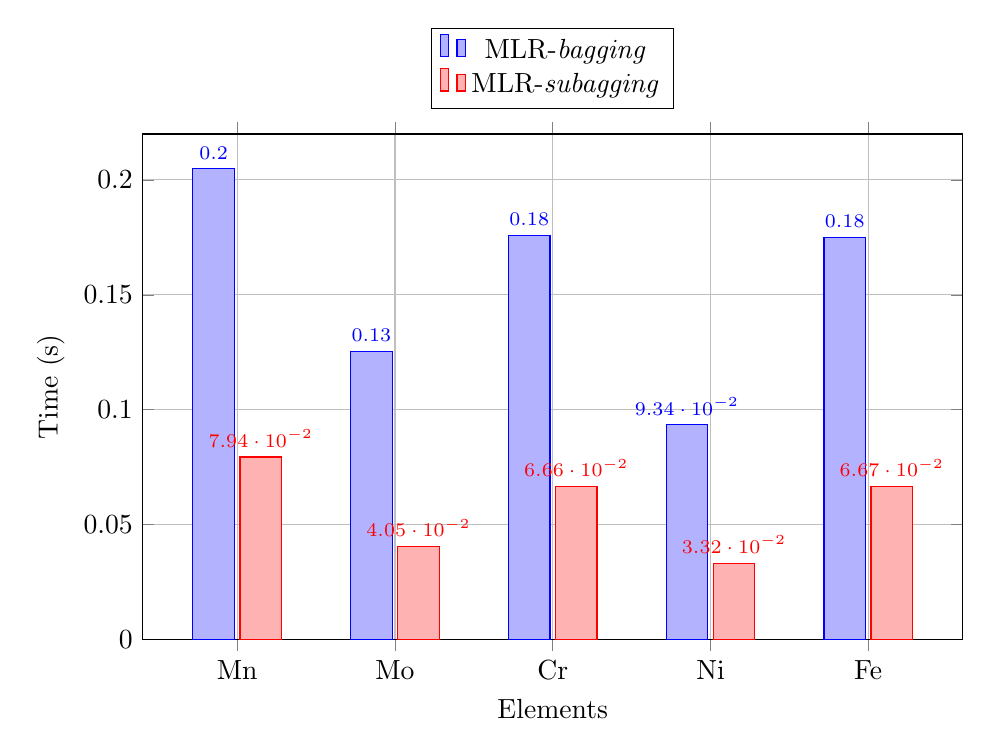
\begin{tikzpicture}
    \begin{axis}[
        ybar,
        width=12cm,
        height=8cm,
        xlabel={Elements},
        ylabel={Time (s)},
        symbolic x coords={Mn, Mo, Cr, Ni, Fe},
        xtick=data,
        legend style={at={(0.5,1.05)}, anchor=south},
        bar width=15pt,
        ymin=0,
        ymax=0.22,
        grid=major,
        nodes near coords,
        nodes near coords align={vertical},
        every node near coord/.append style={font=\scriptsize, rotate=0},
        enlarge x limits=0.15,
        yticklabel style={/pgf/number format/fixed, /pgf/number format/precision=3}
    ]
    
    \addplot coordinates {
        (Mn, 0.2048)
        (Mo, 0.1254)
        (Cr, 0.1757)
        (Ni, 0.0934)
        (Fe, 0.1750)
    };
    
    \addplot coordinates {
      (Mn, 0.0794)
      (Mo, 0.0405)
      (Cr, 0.0666)
      (Ni, 0.0332)
      (Fe, 0.0667)
    };
    
    \legend{MLR-\textit{bagging}, MLR-\textit{subagging}}
    \end{axis}
\end{tikzpicture}
}
%\legend{Source: prepared by the author.}
\end{figure}

MLR-subagging reveals itself as an advantageous alternative in scenarios where processing time constitutes a critical factor and small performance losses are tolerable. The consistent reduction in execution time across all elements demonstrates the robustness of this computational advantage, with time savings ranging from approximately 60\% to 65\% relative to MLR-bagging.

\section{Conclusions}

This study performs a systematic investigation of bootstrap, bagging, and subagging resampling techniques applied to Multiple Linear Regression (MLR) in the context of multivariate calibration of data from alloy steel samples. The comparative analysis between algorithms reveals performance variations associated with the evaluated analyte.

The MLR-bagging and MLR-subagging approaches obtain significant gains in prediction accuracy for Chromium (Cr) and Iron (Fe) elements, evidencing the effectiveness of ensemble techniques in these contexts. In contrast, classical MLR presents superior performance in predicting Manganese (Mn), Molybdenum (Mo), and Nickel (Ni) elements, indicating that for these analytes, the additional complexity introduced by ensemble strategies does not result in significant precision improvements.

Computational efficiency analysis evidences significant differences among evaluated methods. Classical MLR presents the best performance in terms of execution time, configuring itself as the most efficient approach. MLR-subagging occupies an intermediate position, with processing time approximately 2.5 times lower than MLR-bagging, although still between 15 and 20 times higher than classical MLR.

The investigation indicates that MLR-bagging and MLR-subagging approaches are more appropriate for analyzing Chromium (Cr) and Iron (Fe) elements, especially in scenarios where predictive accuracy constitutes an essential requirement. For Manganese (Mn), Molybdenum (Mo), and Nickel (Ni) elements, results support the adoption of classical MLR, due to its simplicity and high computational efficiency.

The trade-off relationship between predictive accuracy and execution time configures itself as a decisive element in technique selection, and should be weighed according to the specific requirements of each application directed to alloy steel analysis. In this context, the present study offers relevant technical subsidies to support informed decisions regarding the choice of the most appropriate method in different application scenarios.

\section*{Acknowledgments}

The authors thank the Instituto Federal de Goiás, Campus Anápolis, for the support provided for this research.

\begin{thebibliography}{99}

\bibitem{Ewing:1972}
Ewing, G. W.; \textit{Métodos Instrumentais de Análise Química}; Edgard Blucher: São Paulo, 1972.

\bibitem{Harley:1954}
Harley, J. H.; Wiberley, S. E.; \textit{Instrumental Analysis}; John Willey \& Sons: New York, 1954.

\bibitem{Skoog:1997}
Skoog, D. A.; Holler, F. J.; Nieman, T. A.; \textit{Principles of Instrumental Analysis}, 5th ed.; Brooks Cole: USA, 1997.

\bibitem{Pimentel:1998}
Pimentel, M. F.; Barros Neto, B.; Araújo, M. C. U.; Coelho, A. L. S.; \textit{J. Autom. Chem.} \textbf{1998}, \textit{20}, 69.

\bibitem{Kramer:1998}
Kramer, R.; \textit{Chemometric Techniques for Quantitative Analysis}; CRC Press: USA, 1998.

\bibitem{Martens:1989}
Martens, H.; Naes, T.; \textit{Multivariate Calibration}; John Wiley \& Sons: USA, 1989.

\bibitem{Lawson:1974}
Lawson, C. L.; Hanson, R. J.; \textit{Solving Least Squares Problems}; Prentice-Hall: USA, 1974.

\bibitem{Draper:1998}
Draper, N. R.; Smith, H.; \textit{Applied Regression Analysis}, 3rd ed.; John Willey \& Sons: USA, 1998.

\bibitem{Johnson:2001}
Johnson, R. A.; Wichern, D. W.; \textit{Applied Multivariate Statistical Analysis}, 5th ed.; Prentice Hall: USA, 2001.

\bibitem{Chatterjee:2006}
Chatterjee, S.; Hadi, A. S.; \textit{Regression Analysis by Example}, 4th ed.; John Willey \& Sons: USA, 2006.

\bibitem{Kupper:1998}
Kupper, A. W. K.; Kleinbaum, D. G.; \textit{Applied Regression Analysis and Other Multivariate Methods}, 3rd ed.; PWS Pub. Co.: USA, 1998.

\bibitem{Stephan:2005}
Stephan, D.; Levine, D. M.; Krehbiel, T. C.; \textit{Estatística - Teoria e Aplicações}; LTC: Rio de Janeiro, 2005.

\bibitem{Efron:1994}
Efron, B.; \textit{The Jackknife, the Bootstrap and Other Resampling Plans}; SIAM: USA, 1994.

\bibitem{Efron:1997}
Efron, B.; Tibshirani, R. J.; \textit{J. Am. Stat. Assoc.} \textbf{1997}, \textit{92}, 548.

\bibitem{Fernandez:1999}
Fernández, J. M. V.; Manteiga, W. G.; \textit{Comput. Stat. Data Anal.} \textbf{1999}, \textit{35}, 211.

\bibitem{Breiman:1996}
Breiman, L.; \textit{Mach. Learn.} \textbf{1996}, \textit{24}, 123.

\bibitem{Shabbir:2024}
Shabbir, M.; Chand, S.; Iqbal, F.; \textit{Commun. Stat. Simul. Comput.} \textbf{2024}, \textit{53}, 3653.

\bibitem{Hong:2020}
Hong, H.; Liu, J.; Zhu, A.-X.; \textit{Sci. Total Environ.} \textbf{2020}, \textit{718}, 137231.

\bibitem{Silva:2020}
Silva, A. C. S.; Oliveira, R. M.; Santos, L. H. S.; \textit{Rev. Estat. Ciênc. Soc.} \textbf{2020}.

\bibitem{Buhlmann:2003}
Bühlmann, P.; \textit{Research Report}, ETH Zürich, 2003.

\bibitem{Revelas:2024}
Revelas, C.; Boldea, O.; Werker, B. J. M.; arXiv:2404.01832, 2024.

\bibitem{Qin:2023}
Qin, T.; Huang, W.-M.; arXiv:2311.02827, 2023.

\bibitem{Galvao:2006}
Galvão, R. K. H.; Araújo, M. C. U.; Fragoso, W. D.; Silva, E. C.; José, G. E.; Soares, S. F. C.; Paiva, H. M.; \textit{Chemom. Intell. Lab. Syst.} \textbf{2006}, \textit{81}, 60.

\bibitem{John:2025}
Eaton, J. W.; GNU Octave, version 9.2.0; Free Software Foundation, 2025.

\end{thebibliography}
\cite{BREIMAN:2001}
\bibliographystyle{plain}
\bibliography{references}
\thispagestyle{empty}%

\end{document}